\chapter{Dokumentacja użytkownika} 
%============================================================================================================================
%							 	Sterowanie w grze
%============================================================================================================================
\section{Sterowanie w grze}
\lhead{Rozdział 1. \emph{Fabuła}}
Astronauta w grze biegnie ciągle do przodu, a osoba sterująca nim ma możliwość wykonania skoku poprzez naciśniecie klawisza spacja. W przypadku kiedy gracz chce wykonać krótki skok, tzn. nie może poczekać aż bohater przestanie się wznosić wtedy z pomocą przychodzi klawisz Ctr którym zatrzymujemy ruch pionowy kosmonauty. Zatrzymanie następuje na ułamek sekundy, jednak naciskając bardzo szybko ten klawisz można sprawić że bohater leci prawie poziomo. Może się to okazać pomocne przy przelatywaniu przez jakieś tunele na mapie. 


\begin{wrapfigure}{left}{0.5\textwidth}
\begin{center}
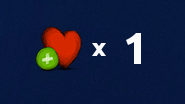
\includegraphics[width=170px]{./Pictures/ilosczycia.png}
\end{center}
\caption{Licznik bonusów}
\label{Etykieta}
\end{wrapfigure}

Podczas biegu na mapie można zebrać bonusy które przywracając pełna ilość życia i sprawiają że życie te nie opada przez kilka sekund. Po znalezieniu takie bonusu w lewym górnym rogu pojawia się informacja o tym. Maksymalnie można mieć 3 niewykorzystane bonusy, i podczas działania jednego nie da się uruchomić kolejnego, co zapobiega zbyt szybkiemu wytraceniu wszystkich znalezionych dodatków. Znaleziony bonus można aktywować poprzez wciśniecie lewego klawisza shift. Po aktywowaniu bonusu dokoła ekranu pojawia się niebieska otoczka oznaczająca nieśmiertelność. 


%============================================================================================================================
%Menu
%============================================================================================================================
\section{Menu}
\lhead{Rozdział 1. \emph{Fabuła}}
Główne menu zostało zaprojektowane w programie do tworzenia grafiki rastrowej Adobe Photoshop. Z jego poziomu można rozpocząć nową grę, kontynuować bieżącą, obejrzeć klawiszologie, oraz listę najlepszych wyników w formie tabelki. Możliwość konstytuowania bieżącej gry staje się aktywna w momencie kiedy gracz podczas gry nacisnął klawisz escape co za skutkowało wyjściem do głównego menu, oraz zamrożeniem bieżącej rozgrywki. Nawigacja w menu odbywa się wyłącznie za pomocą klawiatury. Klawisz strzałka w górę przechodzi do następnej pozycji powyżej, strzałka w dół działa natomiast odwrotnie. Aktualnie wybrany element menu podświetlany jest za pomocą koloru pomarańczowego, nie aktywny kolorem szarym, a domyślny białym. Zatwierdzenie wybranej opcji następuje poprzez wciśniecie klawisza enter, co stanowi standardową nawigacje w większości menu do gier. Naciśnięcie klawisza w głównym menu spowoduje zamknięcie aplikacji. 

\begin{figure}[h]
    \centering
    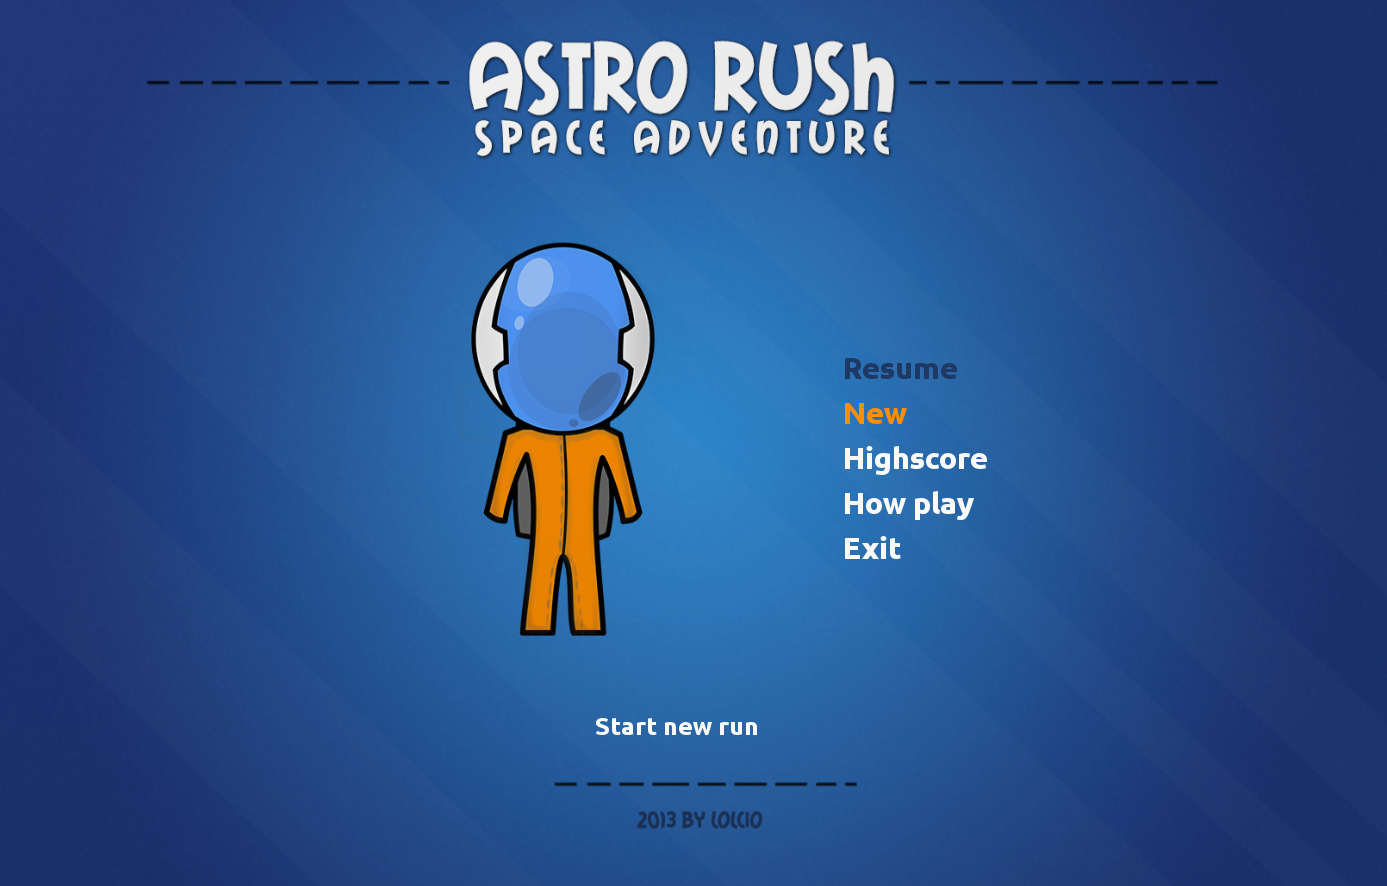
\includegraphics[width=429px]{./Pictures/menu1.png}
    \caption{Menu główne gry}
\end{figure}

\newpage 

\begin{figure}[h]
    \centering
    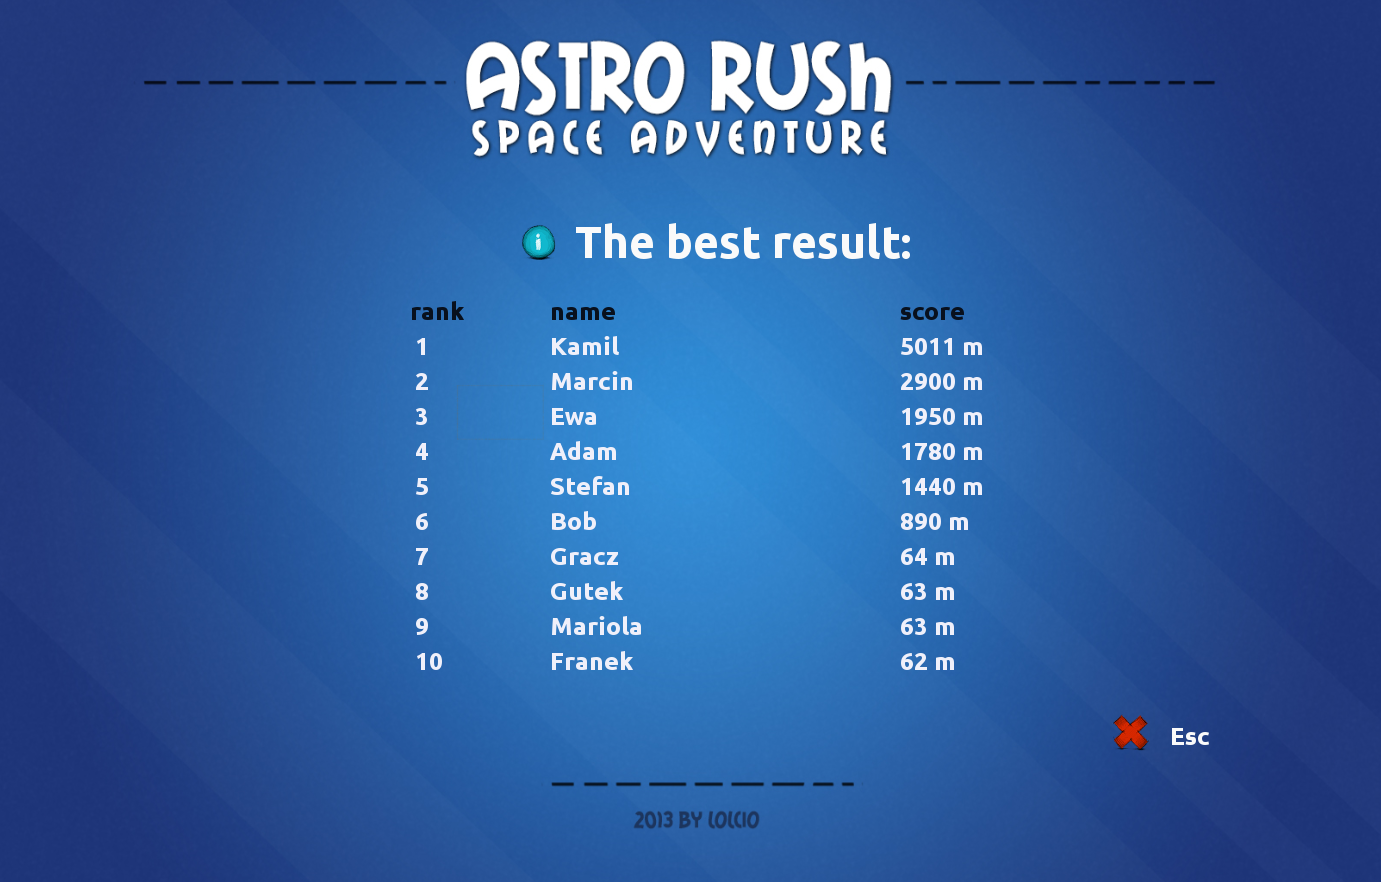
\includegraphics[width=429px]{./Pictures/menu2.png}
    \caption{Highscore w grze}
\end{figure}


\begin{figure}[h]
    \centering
    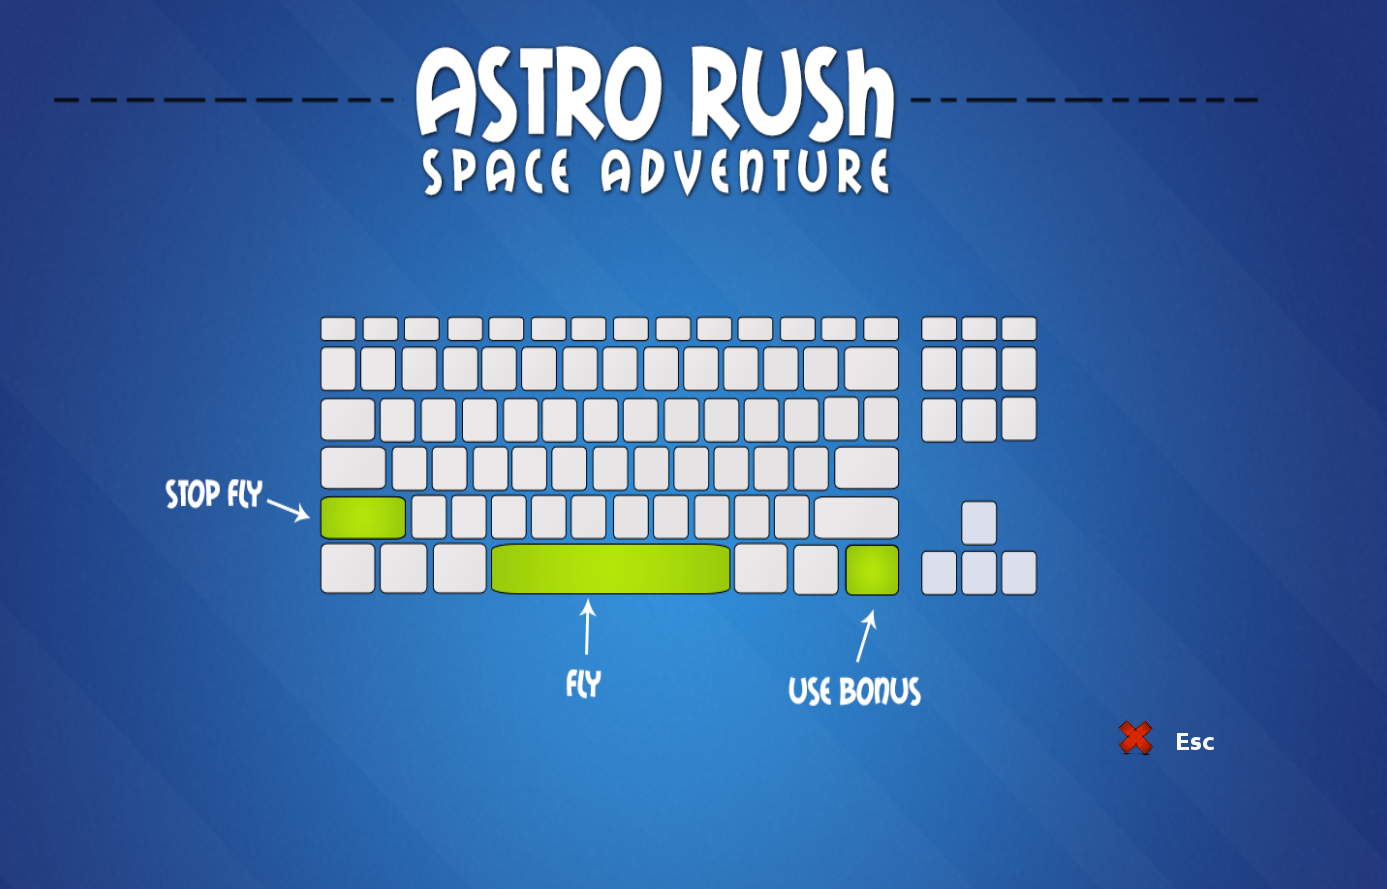
\includegraphics[width=429px]{./Pictures/menu3.png}
    \caption{Klawiszologia dostępna poprzez menu główne w grze}
\end{figure}


%============================================================================================================================
%							 		Instalacja
%============================================================================================================================
\section{Instalacja}
\lhead{Rozdział 1. \emph{Fabuła}}
W tym rozdziale zostanie przedstawiona instalacja potrzebnych bibliotek oraz kompilacja aplikacji na przykładzie dystrybucji Linuksa Debian. W przypadku innych wersji systemu Linuks nie bazujących na Debianie instalacja ta może wyglądać inaczej np. w systemie Fedora gdzie nazwy pakietów są inne, oraz ścieżka do biblioteki SDL jest inna. Dla Fedory kompilacja aplikacja wymaga zmian ścieżek do bibliotek. Dlatego też w przypadku wersji aplikacji który miała by być dostarczona szerszemu gronu odbiorców konieczne jest przygotowanie rozwiązania unifikującego proces kompilacji pod różnymi dystrybucjami Linuksa. Innym rozwiązanie może przygotowanie prekompilowanych pakietów dla najpopularniejszych platform np. deb i rpm. Dodatkowym problemem może okazać się brak niektórych pakietów w repozytorium i konieczność ręcznego ich ściągania, jednak taka sytuacja nie powinna mieć miejsca z racji tego że wykorzystane biblioteki są dość popularne wśród twórców gier. 

W systemie Debian żeby zainstalować wymagane pakiety należy wykonać następujące poleceniem:
\begin{verbatim}
	aptitude install libsdl-dev ######### DOPISAC RESZTE #######
\end{verbatim}

Jeżeli instalacja przebiegła bez problemów to wtedy można przystąpić do kompilowania gry.
W katalogu z rozpakowanym kodem należy wykonać polecenie make i poczekać aż pojawi się informacja o udanym zbudowaniu programu. W przypadku komputerów z wielordzeniowym procesorem można zoptymalizować proces budowania podając parametr -j<tutaj\_liczb\_rdzeni>.

